% -----------------------------------------------------------------------------
% Metodologia
% -----------------------------------------------------------------------------

\chapter{Metodologia}
\label{chap:metodologia}
Com o objetivo de criar aplicações que simulem cada uma das camadas do modelo TCP/IP, foram escolhidos cinco protocolos para serem implementados. Da camada de aplicação o protocolo HTTP, utilizado para comunicação de um sistema final e um servidor Web, permitindo assim navegação pela Internet, será implementado. Da camada seguinte, a de Transporte, devido a sua importância, os dois principais protocolos serão implementados, o protocolo de transporte confiável, TCP, e o não confiável, UDP.
 
Os seguimentos recebidos da camada de transporte deverão ser tratados na camada de internet pelo protocolo IP fazendo uso do roteamento o qual, por sua vez, deverá entregar o datagrama resultante para camada de Enlace. Esta terá o protocolo Ethernet simulado, além do protocolo ARP para tradução do endereço IP para MAC, possibilitando assim o envio do quadro para o host destino.

A Figura \ref{fig:objetivo} representa a arquitetura planejada para o trabalho, na qual os hosts deverão ser conectados pela arquitetura cliente/servidor na camada de Enlace. O sistema deverá, então, ser executado em duas máquinas diferentes, conectadas à mesma rede.


\begin{figure}[H]
	\centering
    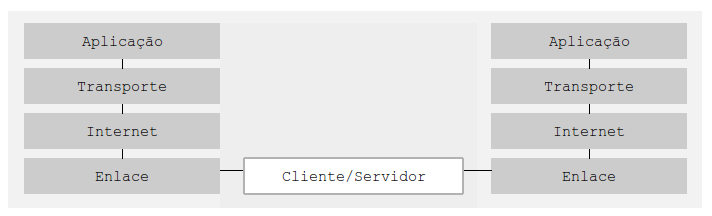
\includegraphics[width=0.80\textwidth]{04-figuras/objetivo.png}
    \caption{Esquema da arquitetura a ser desenvolvida}
    \label{fig:objetivo}
\end{figure}

Cada camada deverá ser implementada de forma independente, e a cada camada, os dados referentes à PDU deverão ser exibidos para, assim, manter a transparência objetivando a utilização deste sistema para o ensino. Estes dados devem seguir a estrutura da PDU de cada camada com os valores de cada campo respectivamente preenchidos.

Objetivando a melhor forma de implementação, considerando a simplicidade e bibliotecas disponíveis, a linguagem utilizada será Python. O desenvolvimento deverá cumprir o planejamento apresentado na Figura \ref{tab:cronograma}, de forma incremental: A primeira camada a ser implementada deverá ser a camada Enlace, para garantir a conexão e transferência correta dos dados. A próxima camada será a de Aplicação, seguida pela camada de Transporte e, por último, a camada de Redes. A cada etapa testes específicos e integrados com as camadas já existentes devem ser feitos para verificar sua validade.


\section{Andamento do trabalho}
A tabela a seguir representa as etapas a serem seguidas durante o desenvolvimento deste trabalho, elaborada no início do projeto e atualizada ao longo de seu desenvolvimento.

\begin{figure}[H]
    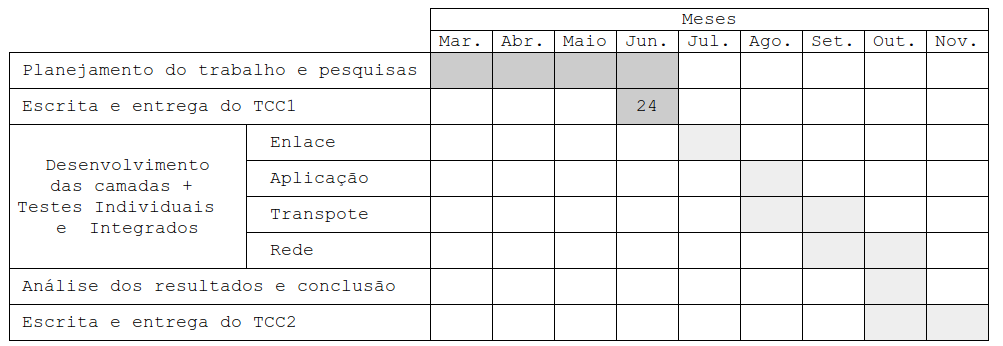
\includegraphics[width=\textwidth]{04-figuras/cronograma.png}
    \caption{Cronograma}
    \label{tab:cronograma}
\end{figure}
